\documentclass[11pt,letterpaper]{article}
\usepackage{graphicx,textcomp}
\usepackage{natbib}
\usepackage{setspace}
\usepackage{fullpage}
\usepackage{color}
\usepackage[reqno]{amsmath}
\usepackage{amsthm}
\usepackage{fancyvrb}
\usepackage{amssymb,enumerate}
\usepackage[all]{xy}
\usepackage{endnotes}
\usepackage{lscape}
\newtheorem{com}{Comment}
\usepackage{float}
\usepackage{hyperref}
\newtheorem{lem} {Lemma}
\newtheorem{prop}{Proposition}
\newtheorem{thm}{Theorem}
\newtheorem{defn}{Definition}
\newtheorem{cor}{Corollary}
\newtheorem{obs}{Observation}
\usepackage[compact]{titlesec}
\usepackage{dcolumn}
\usepackage{tikz}
\usetikzlibrary{arrows}
\usepackage{multirow}
\usepackage{xcolor}
\newcolumntype{.}{D{.}{.}{-1}}
\newcolumntype{d}[1]{D{.}{.}{#1}}
\definecolor{light-gray}{gray}{0.65}
\usepackage{url}
\usepackage{listings}
\usepackage{color}
\usepackage{graphicx}
\usepackage{wrapfig}
\usepackage{relsize}

\definecolor{codegreen}{rgb}{0,0.6,0}
\definecolor{codegray}{rgb}{0.5,0.5,0.5}
\definecolor{codepurple}{rgb}{0.58,0,0.82}
\definecolor{backcolour}{rgb}{0.95,0.95,0.92}

\lstdefinestyle{mystyle}{
	backgroundcolor=\color{backcolour},   
	commentstyle=\color{codegreen},
	keywordstyle=\color{magenta},
	numberstyle=\tiny\color{codegray},
	stringstyle=\color{codepurple},
	basicstyle=\footnotesize,
	breakatwhitespace=false,         
	breaklines=true,                 
	captionpos=b,                    
	keepspaces=true,                 
	numbers=left,                    
	numbersep=5pt,                  
	showspaces=false,                
	showstringspaces=false,
	showtabs=false,                  
	tabsize=2
}
\lstset{style=mystyle}
\newcommand{\Sref}[1]{Section~\ref{#1}}
\newtheorem{hyp}{Hypothesis}

\title{Problem Set 1}
\date{Due: October 9, 2025}
\author{Rosalie LaCroix}

\begin{document}
	\maketitle
	
	\vspace{1cm}
	\section*{Question 1: Education}

A school counselor was curious about the average of IQ of the students in her school and took a random sample of 25 students' IQ scores. The following is the data set:\\
\vspace{.5cm}

\lstinputlisting[language=R, firstline=42, lastline=42]{PS01MyAnswers.R}  

\vspace{1cm}

\begin{enumerate}
	\item Find a 90\% confidence interval for the average student IQ in the school.\\
	
\textsmaller[1]{To determine a 90\% confidence interval, I defined the n as being equal to the 25 students within the sample, and subsequently determined the need for a t-test as the sample is less than 30. In order to determine the bounds of my confidence interval, I needed the mean, standard deviation, and test statistic. To find the test statistic, I ran a two-tailed test using the qt() function. For a two-tailed test, I put in my confidence coefficient of 0.90, subtracted it from 1, and divided the result of that by 2 as I am looking for the critical values on the two tails of the distribution. I defined my degrees of freedom as n - 1, as is standard for a t-test. Taking the test statistic and multiplying it by the standard error (standard deviation/sqrt(n)), I could then subtract that value from or add it to the mean of the sample to determine the lower and upper bounds of my confidence interval. This final step is executed due to the fact that we want to find values on both sides of the mean that are known as our population parameters. These parameters are the values that with repeated sampling we can say will be be in 90\% of confidence intervals.}

\lstinputlisting[language=R, firstline=44, lastline=52]{PS01MyAnswers.R}

\textsmaller[1]{With repeated sampling, 90\% of confidence intervals will contain the population parameters 93.96, 102.92.}
	
	\item Next, the school counselor was curious  whether  the average student IQ in her school is higher than the average IQ score (100) among all the schools in the country.\\ 
	
	\noindent Using the same sample, conduct the appropriate hypothesis test with $\alpha=0.05$.
	
\textsmaller[1]{To begin my hypothesis testing, I set the null hypothesis to be that the average student IQ in the counselor's school is less than or equal to the average IQ score among all other schools in the country of 100. The alternative hypothesis then states that the average student IQ in the counselor's school is greater than the average IQ score among all other schools of 100. The next step was determining the test statistic of t, as the sample size is less than 30. Calculation of the test statistic required the standard error, which can be found by dividing the standard deviation from the previous question by the square root of n. The t-statistic is a measure of how our sample data differs from what is expected in the null hypothesis, which means that to determine this statistic we needed to find the difference between our sample mean and the null hypothesis of 100. This difference is then divided by the standard error to calculate the t-statistic. The standard error, difference in means, t-statistic, and degrees of freedom were all utilized to determine the p-value. I defined my degrees of freedom as n - 1, as is standard for a t-test. It was important to indicate that we were utilizing a one-sided test, as the alternative hypothesis states that the student's IQ is greater than the national average, so we want to know solely about the upper tail. The p-value can be compared to the alpha value of 0.05 to tell us how likely it is that the sample statistic would occur if the null hypothesis were true. A p-value greater than 0.05 tells us that there is not significant evidence to reject the null hypothesis and it is therefore highly unlikely for the sample statistic to occur, whereas a p-value less than 0.05 tells us that there is significant evidence to reject the null hypothesis.}
	
\lstinputlisting[language=R, firstline=66, lastline=78]{PS01MyAnswers.R}

\begin{center}
	\begin{tabular}{ c c c c}
		Diff in Means & Std Error & t & P-Value \\ 
		-1.560 & 2.619 & -0.596 & 0.722 \\     
	\end{tabular}
\end{center}

\textsmaller[1]{The p-value is greater than 0.05, therefore we did not find significant evidence to reject the null hypothesis that the school counselor's school's average student IQ score was higher than the average score among all the schools in the country.}
	
\end{enumerate}

\newpage

	\section*{Question 2: Political Economy}

\noindent Researchers are curious about what affects the amount of money communities spend on addressing homelessness. The following variables constitute our data set about social welfare expenditures in the USA. \\
\vspace{.5cm}


\begin{tabular}{r|l}
	\texttt{State} &\emph{50 states in US} \\
	\texttt{Y} & \emph{per capita expenditure on shelters/housing assistance in state}\\
	\texttt{X1} &\emph{per capita personal income in state} \\
	\texttt{X2} &  \emph{Number of residents per 100,000 that are "financially insecure" in state}\\
	\texttt{X3} &  \emph{Number of people per thousand residing in urban areas in state} \\
	\texttt{Region} &  \emph{1=Northeast, 2= North Central, 3= South, 4=West} \\
\end{tabular}

\vspace{.5cm}
\noindent Explore the \texttt{expenditure} data set and import data into \texttt{R}.
\vspace{.5cm}
\vspace{.5cm}
\begin{itemize}

\item
Please plot the relationships among \emph{Y}, \emph{X1}, \emph{X2}, and \emph{X3}? What are the correlations among them (you just need to describe the graph and the relationships among them)?

\lstinputlisting[language=R, firstline=3, lastline=43]{Plots.R}

\begin{figure}[h]
	\caption{Relationships Among Y, X1, X2, and X3}
	\label{fig:plot_1}
	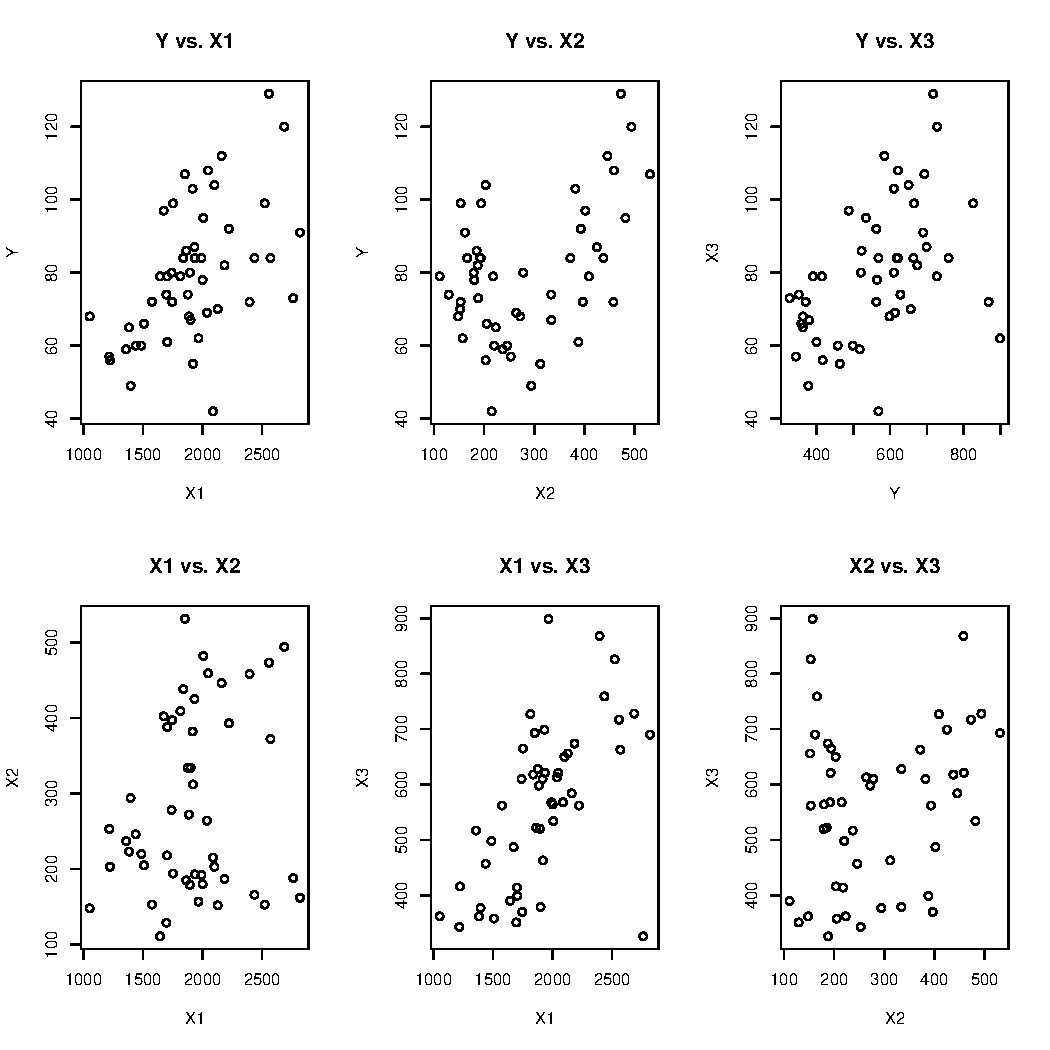
\includegraphics[width=8cm]{six_plots_PS01.pdf}
	\centering
\end{figure}

Y vs. X1
\textsmaller[1]{The graph shows there is a weak to moderate, positive, linear relationship between per capita personal income and per capita expenditure on shelters/housing assistance in states. The reason the relationship is being described as weak to moderate, is that there is a grouping of states that show a stronger positive, linear relationship towards the lower/lower-middle end of the two variables, but as both variables increase, this relationship becomes much weaker.}

Y vs. X2 
\textsmaller[1]{The graph shows that there is little association between states' number of residents per 100,000 that are "financially insecure" and the amount of money that state is spending on shelters/housing assistance. Though the general association appears minimal, it is important to note that there is a weak, negative, linear association between states that have less than 300 residents per 100,000 and their expenditure on shelters/housing assistance. There also appears to be a weak, positive, linear association for states that have greater than 400 residents per 100,000 and their expenditure on shelters/housing assistance. These patterns appear to have a near-parabolic structure.}

Y vs. X3
\textsmaller[1]{The graph shows that there is a weak, positive, linear association between the per capita expenditure on shelters/housing assistance in a state and it's number of people per thousand residing in urban areas. As Y increases, the relationship appears to weaken further.}

X1 vs. X2
\textsmaller[1]{The graph shows that there is a minimal association between states' per capita personal income and the number of residents that are financially there. In states where the per capita personal income is lower, a faint weak, positive association can be seen that begins to spread out as per capita personal income increases.}

X1 vs. X3
\textsmaller[1]{The graph shows that there is a weak to moderate, positive, linear relationship between states' per capita personal income and the number of people per thousand residing in rural areas. The association weakens when the per capita personal income reaches approximately 2300. There is an outlier from the general trend that appears on the higher end of per capita personal income (X1) but falls very low in the number of people residing in urban areas (X3).}

X2 vs. X3
\textsmaller[1]{The graph shows that there is no association between the number of residents that are financially insecure and the number of people residing in urban areas across states.}

\vspace{.5cm}
\item
Please plot the relationship between \emph{Y} and \emph{Region}? On average, which region has the highest per capita expenditure on housing assistance?

\begin{figure}[h]
	\caption{Relationship between Y and Region}
	\label{fig 2:plot_2}
	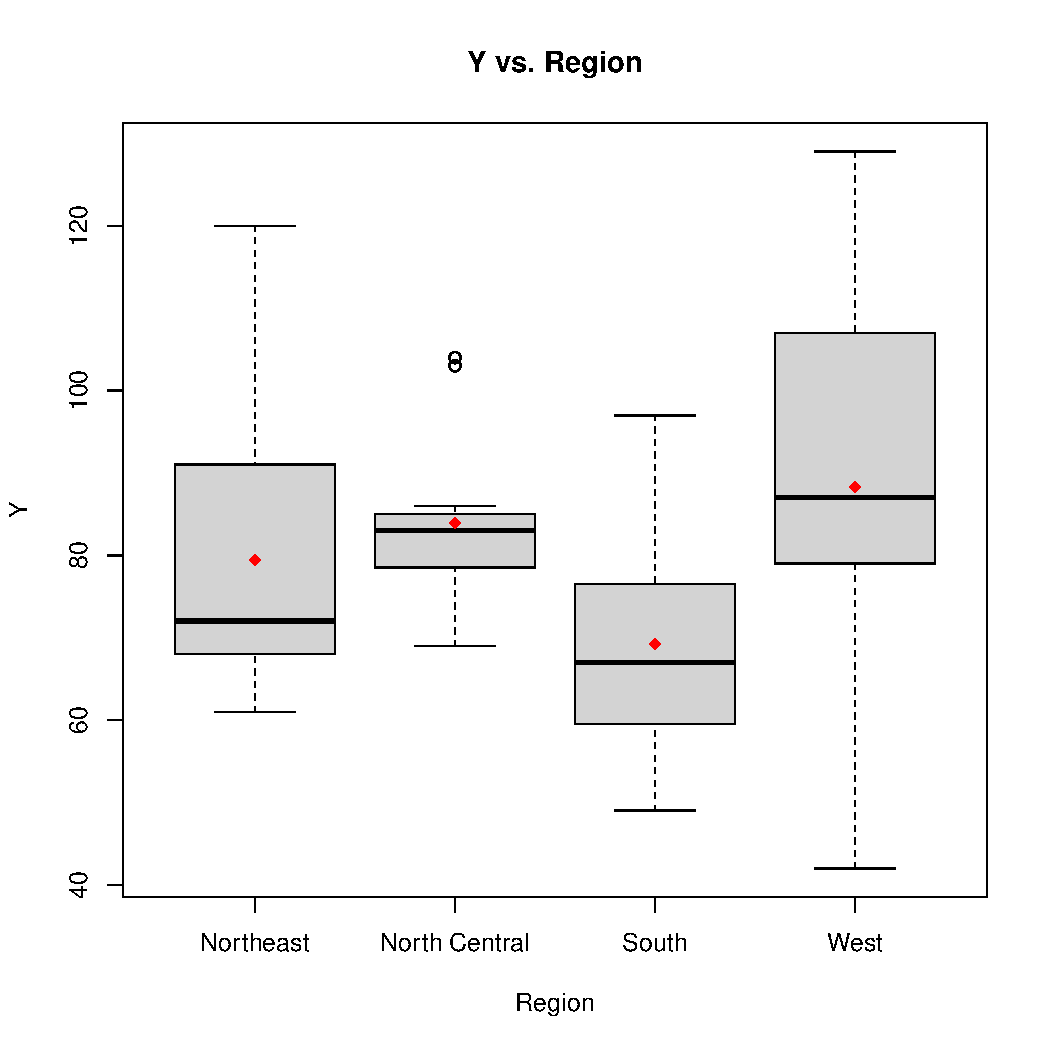
\includegraphics[width=8cm]{y_region_PS01.pdf}
	\centering
\end{figure}

\textsmaller[1]{As you can see in Figure~\ref{fig 2:plot_2}, the West has the highest per capita expenditure on housing assistance. This can be seen in the boxplot with the red dot marking the means of each region.}

\vspace{.5cm}
\item
Please plot the relationship between \emph{Y} and \emph{X1}? Describe this graph and the relationship. Reproduce the above graph including one more variable \emph{Region} and display different regions with different types of symbols and colors.

\lstinputlisting[language=R, firstline=183, lastline=190]{PS01MyAnswers.R}

\begin{figure}[h]
	\caption{Relationship between Personal Income and Spending on Shelters/Housing Assistance in States}
	\label{fig 3:plot_3}
	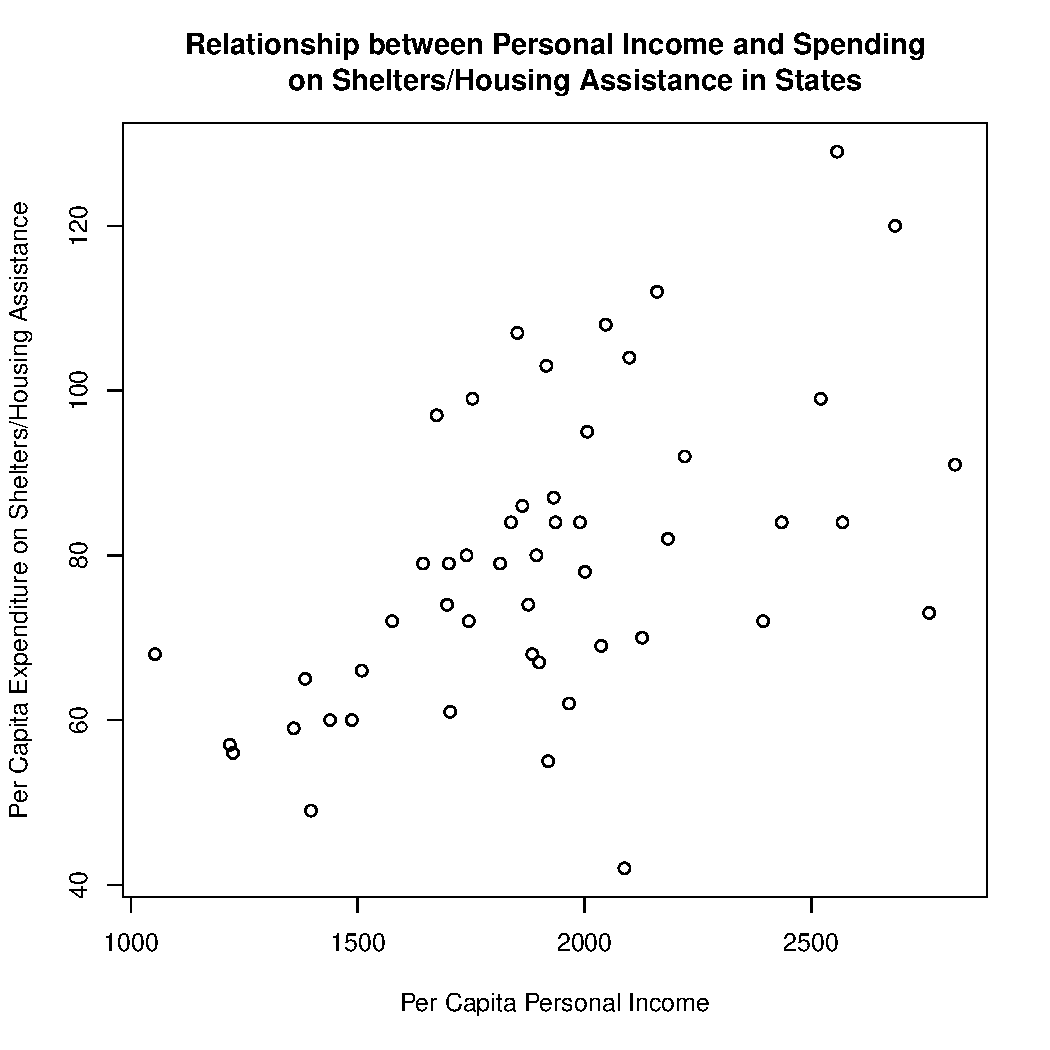
\includegraphics[width=8cm]{original_last_q_PS01.pdf}
	\centering
\end{figure}

\textsmaller[1]{Figure 3 shows there is a weak to moderate, positive, linear relationship between per capita personal income and per capita expenditure on shelters/housing assistance in states. The reason the relationship is being described as weak to moderate, is that there is a grouping of states that show a stronger positive, linear relationship towards the lower/lower-middle end of the two variables, but as both variables increase, this relationship becomes much weaker.}

\lstinputlisting[language=R, firstline=212, lastline=234]{PS01MyAnswers.R}

\begin{figure}[h]
	\caption{Relationship between Personal Income and Spending on Shelters/Housing Assistance in States, including Region Specification}
	\label{fig 4:plot_4}
	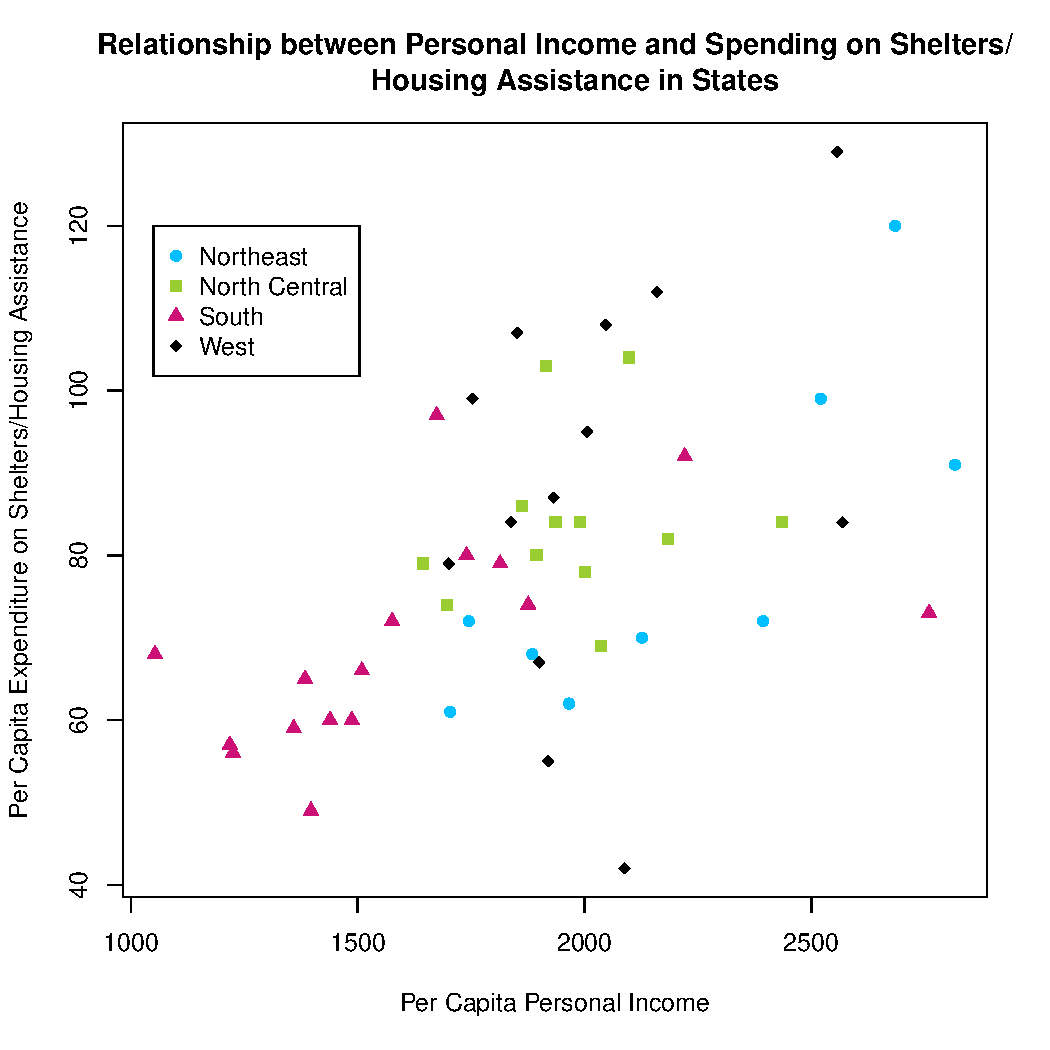
\includegraphics[width=8cm]{last_question_PS01.pdf}
	\centering
\end{figure}
\end{itemize}


\end{document}
